\documentclass[12pt, french]{article}

\usepackage{fancyhdr, fancybox, lastpage}
\usepackage[most]{tcolorbox}
\usepackage[a4paper, margin={0.3in, .75in}]{geometry}
\usepackage{wrapfig}
\pagestyle{fancy}
\renewcommand\headrulewidth{1pt}
\renewcommand\footrulewidth{1pt}
\fancyhf{}
\rhead{ \em{Zakaria Haouzan}}
\lhead[C]{\em{1ére Année Baccalauréat Sciences Expérimentales}}
\chead[C]{}
\rfoot[C]{}
\lfoot[R]{}
\cfoot[]{\em{Page \thepage / \pageref{LastPage}}}


\newtcolorbox{Box2}[2][]{
                lower separated=false,
                colback=white,
colframe=white!20!black,fonttitle=\bfseries,
colbacktitle=white!30!gray,
coltitle=black,
enhanced,
attach boxed title to top left={yshift=-0.1in,xshift=0.15in},
title=#2,#1}


\begin{document}
\begin{center}
   \shadowbox {\bf{Transfert de l’énergie dans un circuit électrique- Puissance électrique }}
\end{center}


%%_________________________Exercice ! :"_________________________Exercice
   \begin{Box2}{Exercice 1 : }
L’énergie électrique reçue par un moteur pendant une durée de $80 min$ est $38 MJ$. La tension d’alimentation du
moteur est $360 V$.
      \begin{enumerate}
      \item Quelle est la puissance électrique du transfert ?

      \item  Calculer l’intensité du courant électrique qui parcourt le moteur.

         \end{enumerate}
   \end{Box2}


%%_________________________Exercice !2 :"_________________________Exercice
\begin{Box2}{Exercice 2 : }
Deux résistances chauffantes $R_1 =25 \Omega$ et $R_2 =50 \Omega$ sont utilisées dans des bouilloires de puissances de chauffe
différentes.
   \begin{enumerate}
   
      \item On les alimente avec une tension de 230 V. Pour quelle résistance l’effet Joule est-il le plus important ?

      \item  Les résistances sont maintenant parcourues par une même intensité de 9,4 A. Comparer leur effet Joule.

      \end{enumerate}
\end{Box2}

%%_________________________Exercice ! 3:"_________________________Exercice
\begin{Box2}{Exercice 3 :}
%\begin{wrapfigure}{r}{0.38\textwidth}
  %\begin{center}
    %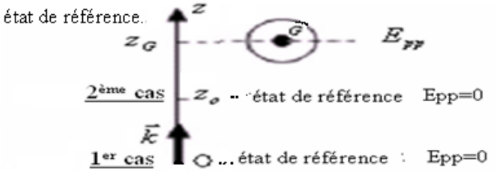
\includegraphics[width=0.38\textwidth]{./img/img00.png}
  %\end{center}
%\end{wrapfigure}
Une batterie d’accumulateur au plomb alimente les lampes d’une automobile. La tension entre les bornes de la
batterie est de $11,9 V$ et l’intensité du courant qui passe dans la batterie est $10,3 A$.
   \begin{enumerate}

\item Quelle est la puissance électrique fournie par la batterie ?

\item Dans ces conditions, le fonctionnement de la batterie dure 17 min. Quelle est l’énergie électrique transférée
dans les circuits récepteurs ? 
   \end{enumerate}
   \end{Box2}

%%_________________________Exercice 4 : _________________________Exercice
\begin{Box2}{Exercice 4 : }
Un générateur G $(U = 6 V)$ débite du courant continu dans un circuit comprenant un résistor de résistance $3\Omega$.
   \begin{enumerate}
\item    Calculer l’intensité du courant qui traverse le résistor.
\item  Calculer l’énergie thermique dissipée par le résistor traversé par le courant pendant $5 min$.
   \end{enumerate}

\end{Box2}

%%_________________________Exercice 5 : _________________________Exercice
\begin{Box2}{Exercice 5 : }
Un récepteur thermique est branché en alternatif sous une tension efficace de 220V. Sa puissance est de $1100W$.
   \begin{enumerate}

   \item Calculer l’intensité efficace I qui traverse le récepteur.
   \item  Calculer la résistance R du récepteur.
   \item  Calculer l’intensité maximale du courant alternatif traversant ce récepteur.
   \item  Ce courant a une période de 20ms, calculer sa fréquence.

      \item Calculer l’énergie consommée pendant 30 minutes de fonctionnement. Exprimer le résultat en Wh.
         \end{enumerate}
\end{Box2}

\begin{Box2}{Exercice 6}
%\begin{wrapfigure}{r}{0.38\textwidth}
  %\begin{center}
    %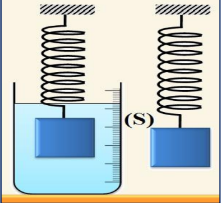
\includegraphics[width=0.38\textwidth]{./img/img02.png}
  %\end{center}
%\end{wrapfigure}
Une génératrice de courant continu convertit une puissance mécanique de $P_m= 1,86 kW$ en énergie électrique.
La tension à ses bornes est de $112V$ et elle débite un courant d’intensité $14,2 A$.
   \begin{enumerate}
   \item Calculer la puissance électrique fournie par cette génératrice.
   \item Calculer la puissance dissipée par effet Joule.
   \end{enumerate}
\end{Box2}

\begin{Box2}{Exercice 7:Exercice Supplémentaire   }
%\begin{wrapfigure}{r}{0.2\textwidth}
  %\begin{center}
    %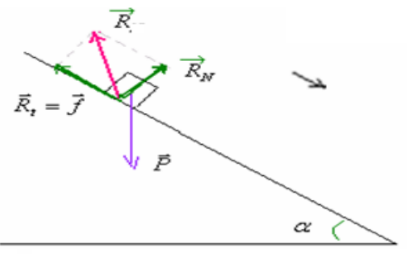
\includegraphics[width=0.2\textwidth]{./img/img03.png}
  %\end{center}
%\end{wrapfigure}
Une batterie d’accumulateur au plomb est chargée de $40 Ah$.
   \begin{enumerate}
   \item La batterie se décharge complètement en $1 h$. La tension au cours de cette décharge est $11,8 V$. Quelle est
l’énergie électrique fournie ?
\item On utilise la batterie pour démarrer une automobile pendant $1,5 s$. La batterie est alors traversée par un
courant d’intensité $0,2 kA$ et la tension à ses bornes est de $10,2 V$.
         \begin{enumerate}
            \item Quelle est l’énergie électrique fournie ?
            \item Quelle est la puissance électrique ?
         \end{enumerate}
   \end{enumerate}
\end{Box2}

\begin{Box2}{Exercice Supplémentaire }
Le champ électrique atmosphérique sous nuage orageux est de l'ordre de $20kV/m$. En moyenne, un éclair
transporte $Q=5 C$. Les nuages d’orages se situent en moyenne à 5000 m du sol.
Un éclair dure en moyenne $25ms$
   \begin{enumerate}

   \item Quelle est la tension U entre le sol et le nuage
   \item Quelle est l’énergie et la puissance d'un éclair d'orage?
   \item Un orage a un nombre d'éclairs très variable, entre 10 et plusieurs milliers. Disons en moyenne 100 éclairs.
      \begin{enumerate}
            \item Quelle est l'énergie moyenne produite par un orage ?
\item Il y a environ $1 million$ d'éclairs par an. Sachant que un foyer consomme une puissance moyenne de $4 kW$
Quel est le nombre d'habitants que cette énergie pourrait alimenter en électricité pendant un an ?
      \end{enumerate}
   \end{enumerate}
\end{Box2}


\vspace{2cm}
\begin{center}
   \Large{ \em{}}
\end{center}



%%_________________________Exercice 6 : _________________________Exercice
\end{document}
